#----------------------------------------Example of Diagram for Lectures and Posters------------------------------
\documentclass[border=10pt]{standalone}
\usepackage[edges]{forest}
\usepackage{tikz}
\usepackage{tikz-qtree}

\begin{document}
%-----------------------------------------Diagram 1----------------------------------------------------------
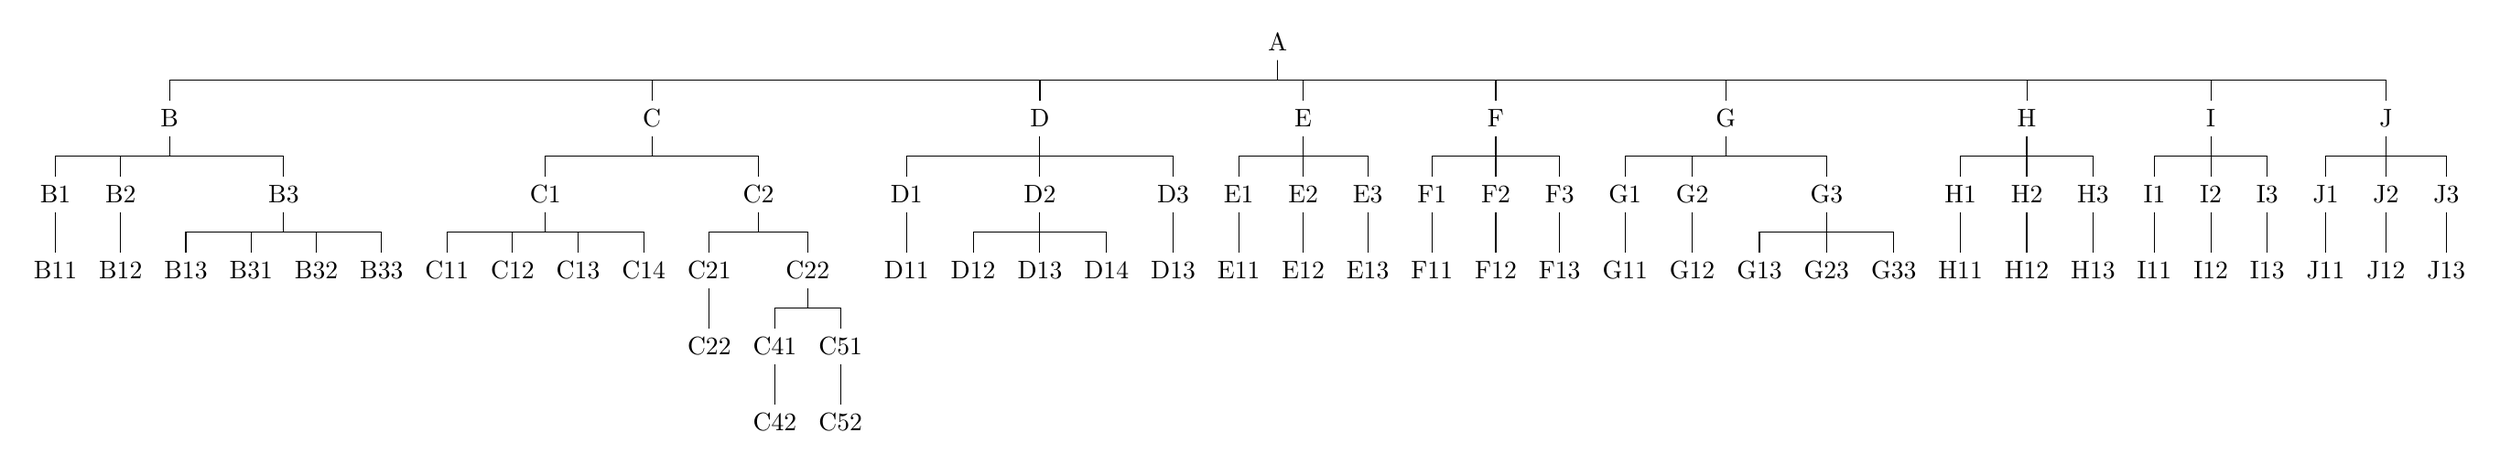
\begin{tikzpicture}
\tikzset{edge from parent/.style={draw,edge from parent path={(\tikzparentnode.south)-- +(0,-8pt)-| (\tikzchildnode)}}}
\Tree [.A 
[.B [.B1 B11 ] [.B2 B12 ]  [.B3 B13 B31 B32 B33 ] ]
[.C [.C1 C11 C12 C13 C14 ] [.C2 [.C21 C22 ][.C22 [.C41 C42 ] [.C51 C52 ] ] ] ] 
[.D [.D1 D11 ] [.D2 D12 D13 D14 ] [.D3 D13 ] ]
[.E [.E1 E11 ] [.E2 E12 ] [.E3 E13 ] ]
[.F [.F1 F11 ] [.F2 F12 ] [.F3 F13 ] ]
[.G [.G1 G11 ] [.G2 G12 ] [.G3 G13 G23 G33 ] ]
[.H [.H1 H11 ] [.H2 H12 ] [.H3 H13 ] ]
[.I [.I1 I11 ] [.I2 I12 ] [.I3 I13 ] ]
[.J [.J1 J11 ] [.J2 J12 ] [.J3 J13 ] ]
]
\end{tikzpicture}

\end{document}
